\chapter{Architecture Exploration and Constraining}

\todo{- Idea concerning structuring the design choices: a previous chapter, context maybe, should talk about the requirements such as 16B elements and 8 write ports. Those two things drive all other design choices. Then instead of calling this chapter design choices, maybe call it '(APL) architecture exploration and constraining' or something like that. Then first approach it from a high level with a section on the initial bandwidth and buffer size proof. Show a figure of the bandwidths between AFU, APL and TLX. Then make clear that the cache has to be split in two levels due to a conflict in design optimization (area versus performance, BRAM gets too full, but there is also URAM available). From there each of the sub-blocks can be discussed, thus OpenCAPI handler, L2 and L1. Again include an updated figure of the high level design and bandwidths etc. The core driver within L2 and L1 is the architecture of the URAM and BRAM arrays. For example, L1 section should start with discussing the architecture of the BRAMs (similarly for L2 the URAMs), since this drove the rest of the design. Then each of those sub-block sections start with a parametrized design of that subblock and each subsection talks about how L1 for example is designed. Then the final subsection for each block talks about constraining this parametrized design from the first subsection.
}

\todo{use axi instead of opencapi interface. axi makes my work portable. may also be used for capi 2.0 for example. opencapi to axi will be built anyway because of confidential slides from xilinx which say that axi will be fpga industry standard.
}

\section{High-level Block Diagram}
\todo{- start by showing high level interaction between TLX, APL and AFU, with APL consisting of OpenCAPI interface, L2 and L1. add figure of it too.\\
- mention the upcoming sections and that they talk about different parts of the APL.\\
- have to mention somewhere the rationale for splitting the cache structure in two levels.\\
- show how AFU, L2 and L1 interface with each other, so parametrized N URAM blocks for L2 and parametrized M BRAM blocks for L1.\\
- by allowing more channels (thus decreasing the number of streams per BRAM/URAM block) between L2 and L1 you increase the number of wiring, so we need to find an optimum between wiring and not stalling L1.\\
- also some rationale about the architecture of the BRAM arrays. we looked into having not to duplicate the data but that didnt work out and posed read and write conflicts. a solution was to add logic for combining requests that can be combined, but that is a lot of logic, while the APL should be as small as possible.\\
- point out that each stream is looked at as a way in terms of an associative cache.\\
}

\begin{figure}[H]
	\centering
	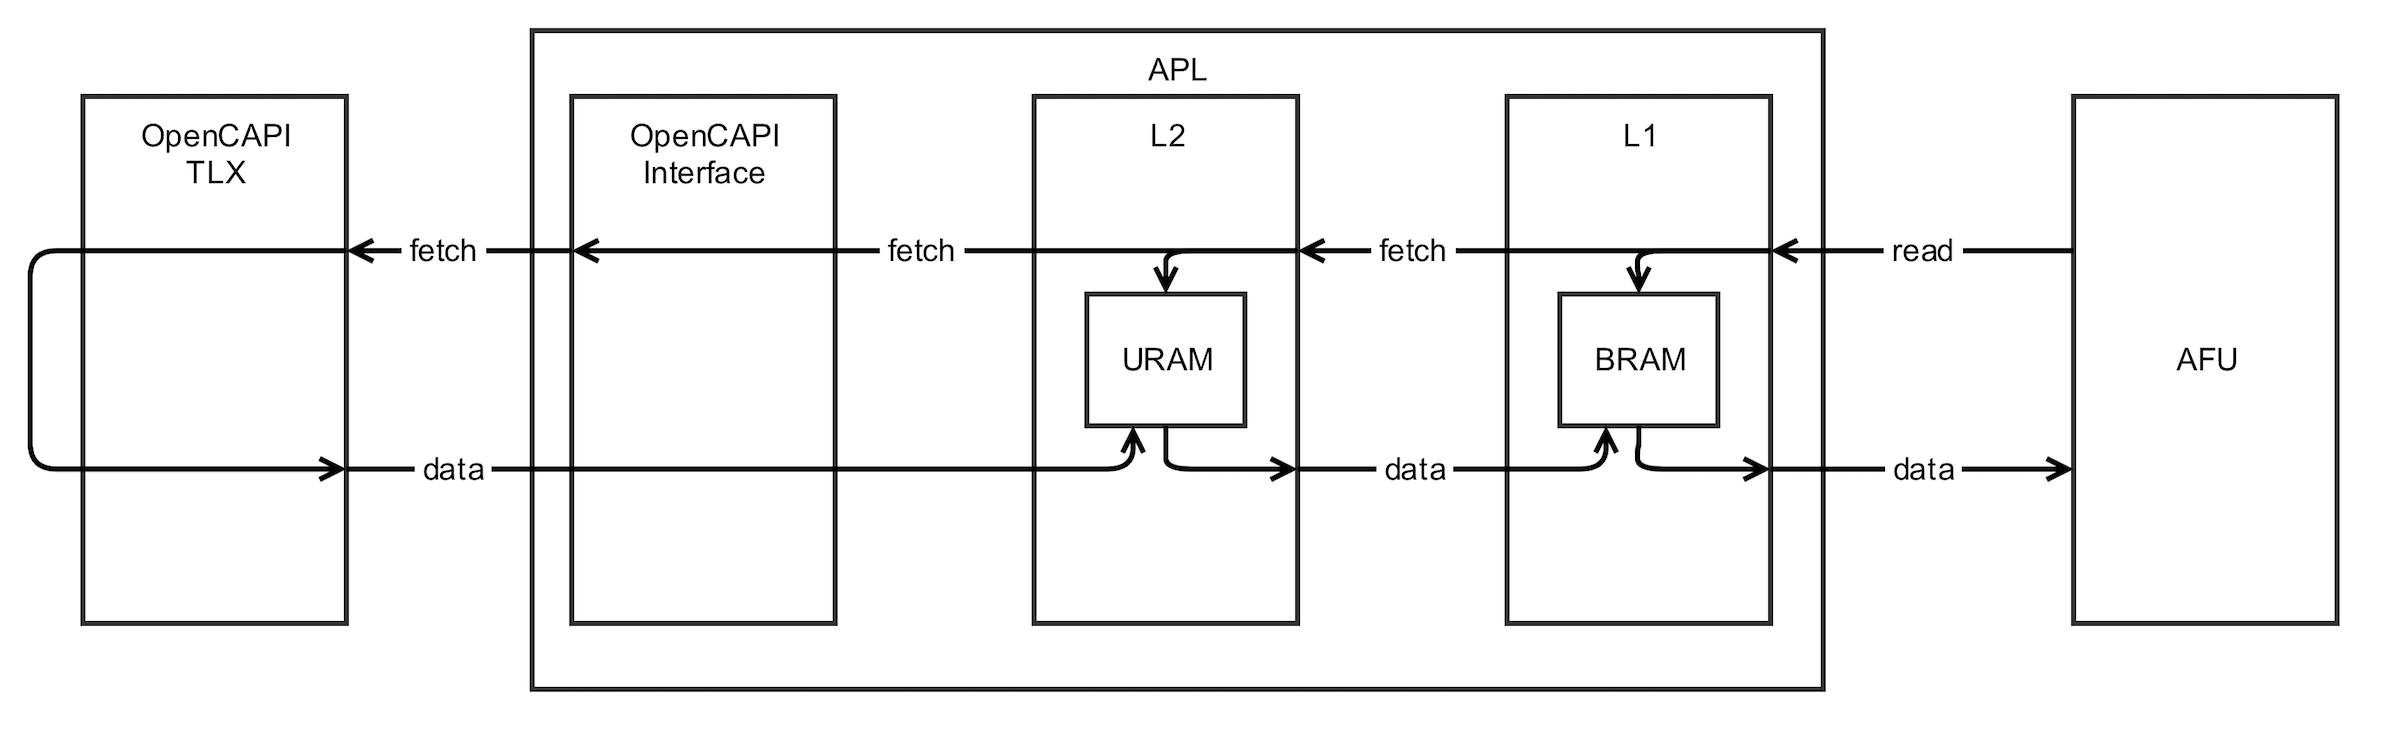
\includegraphics[scale=0.35]{4-dataflow.png}
	\caption{High-level block diagram of the data flow between the AFU, APL and TLX.}
	\label{fig:dataflow}
\end{figure}

\todo{Use colors to show the three 'loops' in this data flow diagram.}

The following three data flows are shown in \autoref{fig:dataflow}.
\begin{itemize}
	\item AFU-L1: The AFU sends read requests to L1 and L1 supplies the corresponding 16 byte elements from the BRAM array.
	\item L1-L2: If the last element of a cache line in L1 is read, a fetch request for the next cache line for that stream is sent to L2. L2 is idle until it receives a fetch request, after which it will read the cache line from the URAM array and sends it to L1.
	\item L2-TLX: When L2 receives a fetch request from L1, it will also send a fetch request to OpenCAPI to fetch a new cache line from the main memory on the host.
\end{itemize}
In order to provide the AFU with data and not stall, each level of cache has to be able to cover the fetching latency. This latency increases the further away from the AFU a new cache line has to be retrieved from.

\subsection{Map Main Memory into Streams}
In a general sense, there are two ways to map the main memory on the host into a number of streams into the stream cache. Basically there are a number of streams $N$, which you would call sets in cache terminology. Then each set has a number of
\begin{itemize}
	\item Consecutive: decide on a number of consecutive cache lines that belong to one stream. After the offset bits in the address, the next log2(number of cache lines per stream) decide on the line within the stream and the next log2(N) bits are to identify the stream.
	\item Interleaved: in this case, the position of the line and set bits are swapped.
\end{itemize}
When using consecutive, it might be that some engines are finished earlier than others and in the end, all end up working on the same stream of data.\\
When using interleaved, if this happens, the engines will deplete stream by stream.

What are the up- and downsides of either approach, when taking 8 read ports into account?

In order to not have to check $M$ (for $M$-ways) tags in parallel for a hit, each cache line can only go to one place in a set (CAM would be used in practise for an associative cache. Not sure how you would do that on a FPGA). So there is a notion of sets with multiple cache lines in each, but each cache line can only go to one place.

\subsubsection{Private versus Shared Cache}
Due to the architecture, both L1 and L2 are the same type of cache as in, either both are private or both are shared.\\

Pro of shared cache is that if an engine finishes early, it can help other engines.\\

Shared or Private Last-Level Cache? Section in book Memory Systems, Cache, DRAM and Disk. Also has additional reference in there.\\
If the target multi-threaded applications exhibit little or no sharing, and the threads have similar working-set sizes, a simple “SMP on a chip” strategy may be the best approach. In such a case, each core has its own private cache hierarchy.\\
If the target multi-threaded applications exhibit a significant amount of sharing, or if the threads have varying working-set sizes, a shared-cache CMP is more attractive.\\









\section{Design of the L1 Cache}
\todo{- show how we got to 16 lines per stream in L1.\\
- show from a high level how L1 interfaces with the AFU (note on post-it) and the assumptions that are made in this model (straightforward model with no tag check, assumption is always hit in L1). this model is used to determine how many streams can be in a bram without stalling. this depends on if you can supply those brams with enough new lines. there are a number of parameters determining the optimum such as streams/bram slice, lines/stream/bram slice, fetch req latency, cycles of staging, total number of streams (=64 high number due to large bandwidth of 25.6GB/s=128B/cycle@200MHz) etc. constrain the design space by constraining parameter by parameter.\\
- show that 8 streams per bram result in no compromize design. illustrate the access patterns considered (for both 8 \& 16 streams. or maybe with smaller examples)\\
- show that 16 streams per bram result in a compromized design (but utilize the brams 100 percent instead of 50), but show that the limitations (= cases that will stall) are very rare cases and follow a weird access pattern.\\
- finally show that staging can fix the 16 stream case and introduce a new equation to take the staging into account. staging is also useful for adding the tag structure.\\
- during implementation, test if these amount of cycles latency calculated are correct.\\
- since it is a stream based cache and not a random access cache, we know what the next cache line requested per stream will be and can therefore easily prefetch\\
}

The following text assumes that the rationale behind using two levels of cache and behind the eight duplicate BRAM arrays in L1 is known to the reader.\\

\autoref{fig:l1} shows a high-level block diagram of how read requests by the AFU are handeled in the L1 cache. In this figure, a rectangle with a triangle on the bottom represents sequential elements and a cloud represents (in this case waiving flag icon) combinatorial elements. The meaning of the letters used in \autoref{fig:l1} are summarized below.
\begin{itemize}
	\item $E$: represents the number of elements present per cache line. The MUX can select one element from a cache line per cycle.
	\item $F$: represents the number of fetch cycles. It indicates how many cycles are needed from issuing a fetch request to L2 for a new cache line, getting it back and written it in L1.
	\item $R$: represents the number of read ports, which is equivalent to the maximum number of read requests issued by the AFU per cycle.
	\item $S$: represents the number of staging cycles. It indicates how many cycles are needed for calculating the BRAM slice addresses and updating the stream pointers (more on this later).
\end{itemize}
The following subsections explain the role of each sub-block, starting from the AFU's point of view. The last section constraints the design space for the L1 cache by modeling \autoref{fig:l1}.

\begin{figure}[H]
	\centering
	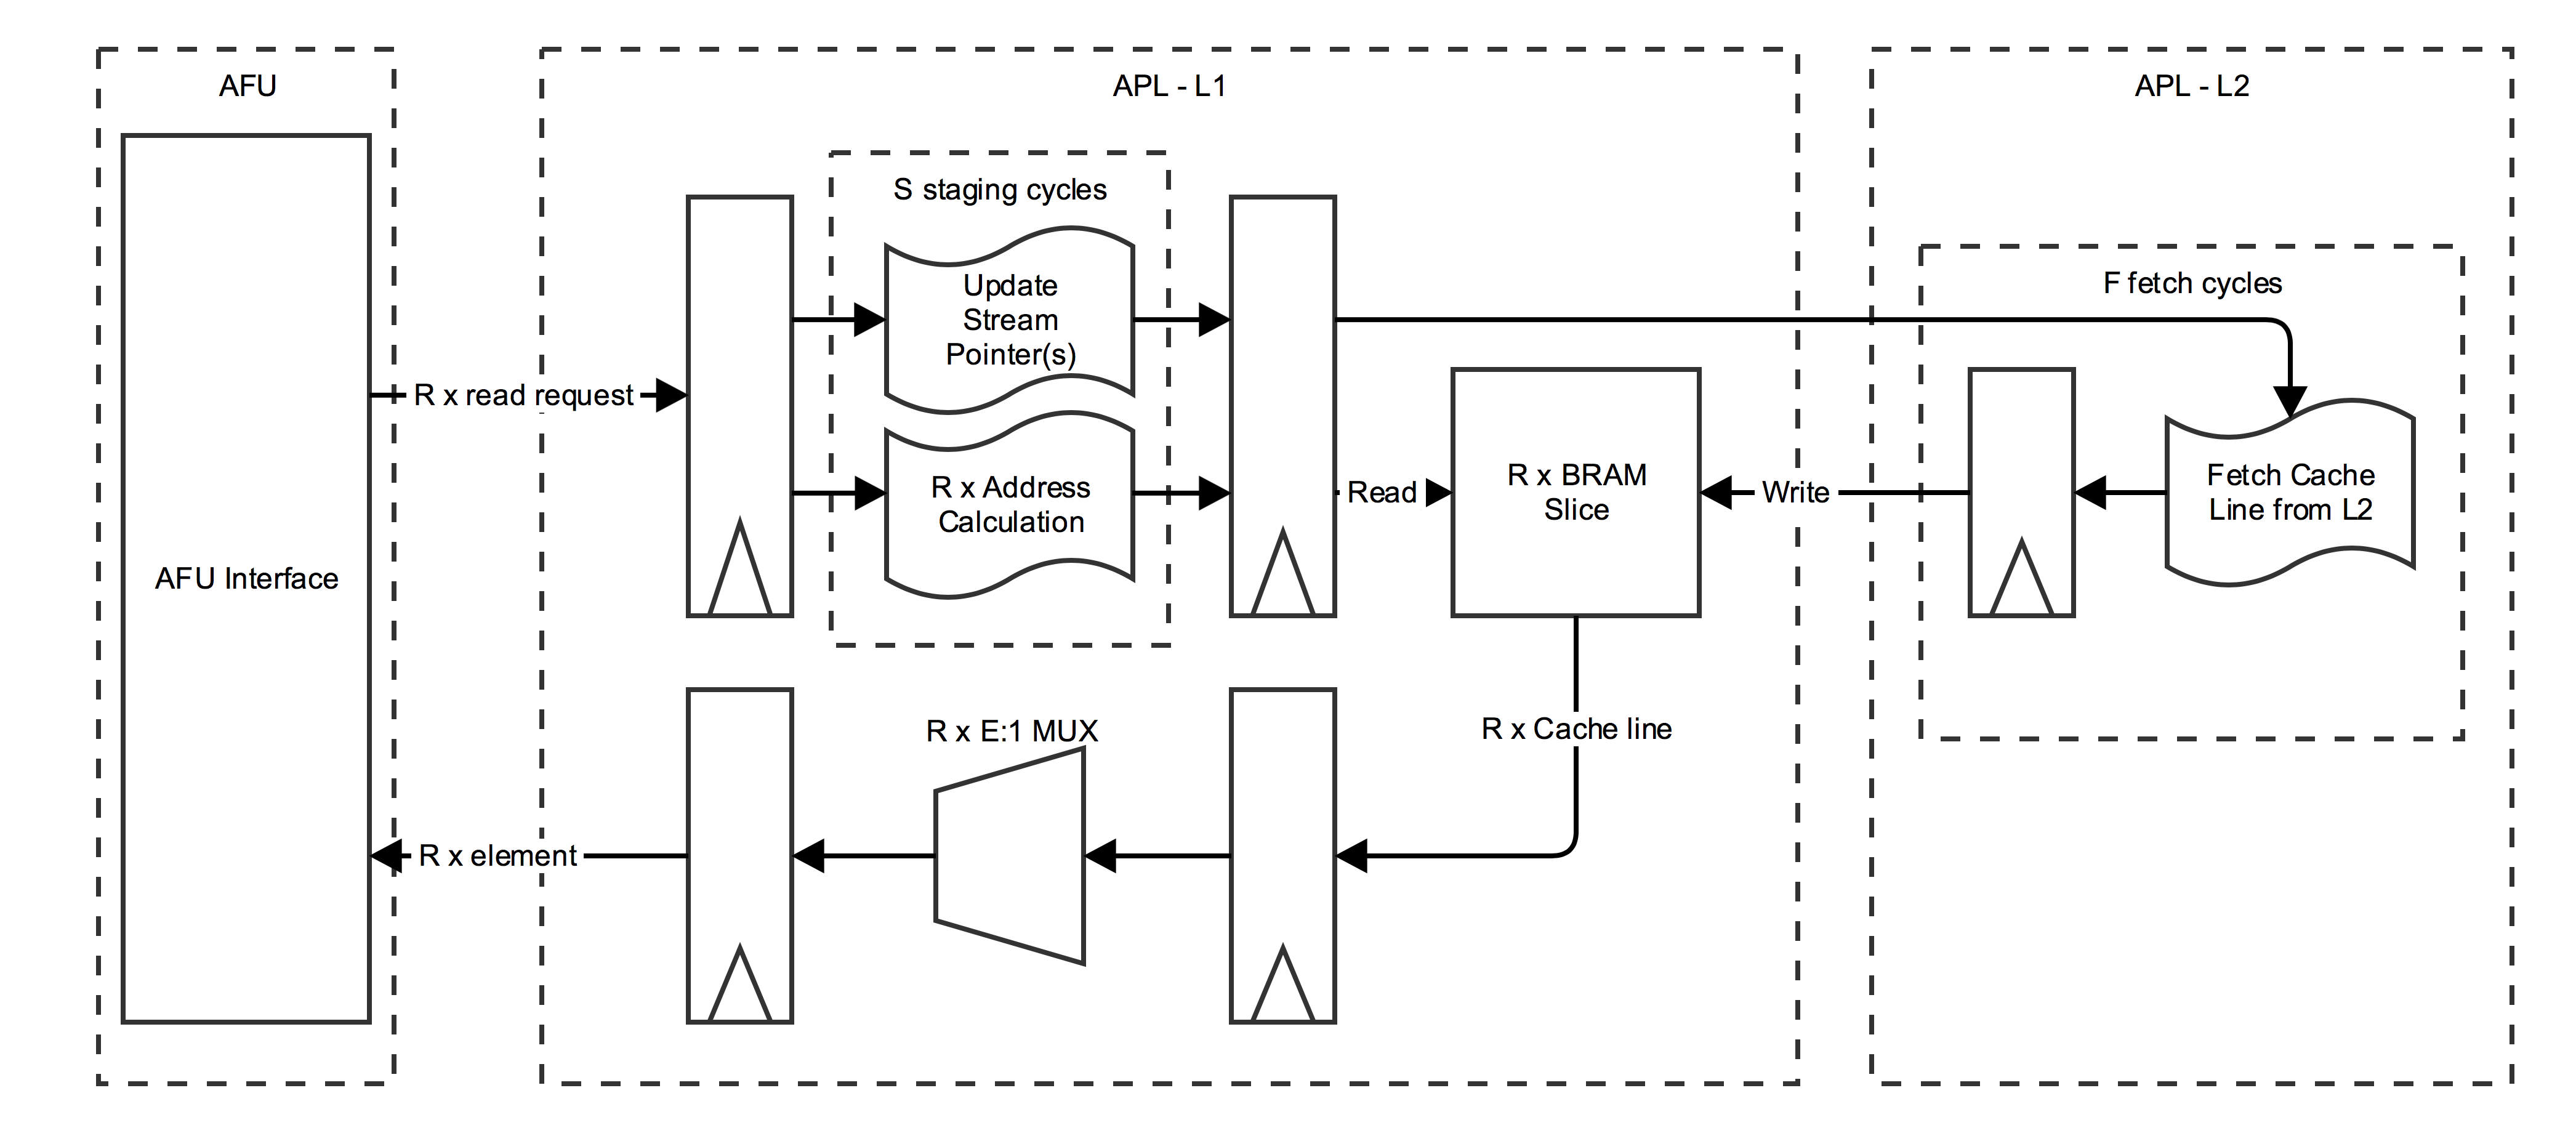
\includegraphics[scale=0.1]{4-l1_cache.png}
	\caption{High-level block diagram of AFU read request handling by the L1 cache.}
	\label{fig:l1}
\end{figure}

\todo{MUX select signal should be drawn in Figure. Is AFU read request.offset for each request.}
\todo{The part where L2 fetch requests are sent should be designed in more depth. For example, 8 fetch requests might be sent out in a cycle. Have to combine them into one L2 fetch queue. So merge 8 fetch queues into one. In the model later one, I assume stream 0 will always be written first etc. So there should be a priority to always let that queue go first. I think this also works for the 16 streams/BRAM case. Then instead of writing stream 0, stream 1, ... stream 15, it will be done as stream 0, stream 8, stream 1, stream 9 etc. In that case, stream 15 is still the last stream to be written, so still the worst case is the same.}

\subsection{AFU Read Requests}
As shown above, the L1 cache sits between the AFU and the L2 cache. The AFU sends as many read requests per cycle to L1 as there are read ports $R$. A certain amount of cycles later ($S+3$), L1 supplies the corresponding requested data to the AFU. Each read request consists of the following four parameters.
\begin{itemize}
	\item \texttt{way\_id}: the way identifier is analogous to a stream identifier. Used for selection of the next cache line in the stream referred to.
	\item \texttt{offset}: the offset determines which element in the cache line is requested.
	\item \texttt{uid}: the unique identifier (UID) is used to match a made read request from the AFU to data returned by the L1 cache.
	\item \texttt{tag}: the tag is used to check if the cache line present in L1 results in a cache hit or miss.
\end{itemize}

\subsection{Address Calculation and Updating Stream Pointers}
\todo{talk about how the calc addr and update pointers work. update pointers should be done at least in the cycle before accessing the BRAM in order to represent the current state of the BRAM to the read requests. dont talk about staging yet. that is done when we plug in numbers into the equations.}

The second block consists of two operations executed in parallel. First of all the corresponding addresses to each read request from the AFU have to be calculated. These addresses are then used to read the requested cache line from the BRAM slice corresponding to that read port.

\todo{this block needs some more thinking. how about calculating the addresses for different read ports if reading 8 elements of the same cache line, but over a cache line boundary. then certain reads are on one line and others on line+1.}
\todo{show parametrized figure of this adder for stream pointer updating}

For addr calc you need wayid and offset from read req. read addr for bram is clog2(total lines in bram = streams/bram * lines/stream).\\
Stream pointers are global to all BRAM slices, thus to all read ports.\\
In total, there are as many of stream pointer update units as there are read ports.\\

A stream pointer is a combination (contatination) of a line and offset. A stream pointer points to the first unread element of each stream. It is used to calculate the address for the next BRAM slice read and it is used for updating the stream pointers to a new value, taking all possible 8 read requests from the AFU into account.

\todo{think about the pointers. how will a write from L2 know at which address it should write? maybe keep a FIFO with addresses per stream?}

\subsection{BRAM and Offset Selection MUX}
\todo{- talk about BRAM and offset selection MUX.\\
- show parametrized version of BRAM slice.\\
- why use SDP instead of TDP?\\
- BRAM config limits.\\
- show double pump limits of BRAM configs as well\\
}

\subsection{Constraining the Design Space}
\todo{- talk about model to constrain the design and its parameters.\\
- some parameters are rather straightforward, such as 8 read ports. mention these just in plain text.\\
- mention somewhere earlier that a fetch request will be sent after reading all elements from a cache line. so only read when there is room.\\}
\todo{LATEST SECTION STRUCTURE IDEA june 18:\\
- should start by mentioning the earlier mentioned max amount of outstanding fetch requests O max equation\\
- then introduce this model for constraining the design.\\
- then doing the actual contraining, where i mention that you should start from looking at the brams and using them most efficiently. from there you can conclude that 16 streams per bram will fill up the brams (after showing 16 lines per stream will be stored in L1). However, it also does not cover all access patterns, so then introduce both staging and using 8 cache lines per stream.\\
- make a final decision on this, which is 16 streams per bram to use the brams more efficiently. support this claim by showing the probability of a stall.\\}

In order to supply the AFU with $R$ elements of data per cycle, the L1 cache has to stay filled while the AFU is allowed any order of streaming access pattern across the different streams. The previous subsections introduced various parameters concering the L1 cache. In this subsection these parameters will be constrained to finalize the L1 cache design. In order to constrain the design of the L1 cache, a model according to \autoref{fig:l1} is constructed.\\
One of the global design goals is to allow for 8 read requests in parallel by the AFU. Therefore the $R$ parameter is equal to 8. Similarly, the size of a single element is 16 bytes. Since the cache line size of the POWER9 processor is 128 bytes, parameter $E$ is equal to 8.\\
Furthermore there are only a finite amount of BRAM configurations available, as mentioned earlier. This limitation constraints the possible configurations of a BRAM slice.\\

\subsubsection{Maximum Number of Outstanding Cache Line Writes}
The maximum number of outstanding cache line writes, denoted by $O_{max}$, depends on $F$, the number of fetch cycles, on the maximum number of fetch requests issued per cycle, which is equal to the number of read ports $R$ and on $B$, the number of streams per BRAM. The maximum number of outstanding cache line writes occurs for example (assuming L1 starts in a completely full state) in the case where every read request from a single cycle results in a fetch request to L2, times the amount of cycles this can be consequtively sustained. This is equal to $B$. Then, there is an overlap in fetch request cycles $F$ if the previous statement can be sustained for two or more consequtive cycles. Therefore, even though some fetch requests are still made, the first fetch requests has been written into the BRAM (right hand side part between brackets).
\begin{equation}
	% O max = latency + total streams/bram / number of read ports * maximum amount of new fetch reqs / cycle - (total streams/bram / number of read ports - 1)
	% O max = F + B / R * R - (B / R - 1) = F + B - (B / R - 1)
	O_{max} = F + B - (\frac{B}{R} - 1)
\end{equation}
\todo{if staging is taken into account, the max number of outstanding writes increases, thus the buffer size increases. another constraint to be taken into account to use the buffers (FIFOs) as efficiently as possible.}

\subsubsection{Number of Lines per Stream}
\todo{Why are 16 lines per stream needed?}
$L$ stands for the number of lines per stream.\\
Therefore, parameter $L$ is equal to 16.\\

\subsubsection{BRAM}
Each BRAM will be double pumped such that each BRAM can hold a single element of 16 bytes. In that case, a single 36K SDP BRAM can hold up to $256/L=16$ streams. The number of streams per BRAM slice is denoted by paramter $B$ and is equal to 16 in this case. Even though each BRAM can hold up to 16 streams, the limiting factor here is the write bandwidth. Each cycle, only one new cache line can be written into a BRAM slice, while up to 8 fetch requests can be made. Therefore, if no compromises are allowed and maximum bandwidth (25.6GB/s) is desired, parameter $B$ can also be decreased to 8 instead of 16, which implies twice as many BRAMs (52 percent utilization on the KU15P) and also half-full BRAMs. This will increase the amount of wiring between L1 and L2 from 4K to 8K (if the total amount of streams are 64), but has the advantage of being able to write 8 cache lines per cycle to the BRAM slices instead of 4 cache lines per cycle. It shows a trade off between stalls and resource utilization of the fpga (bram 50 or 100 percent full and 8k or 4k wires from uram to bram).\\
In order to decide on the amount of streams per BRAM slice, a model of \autoref{fig:l1} is constructed. Two additional parameters come into play, $F$ and $S$, which are shown in \autoref{fig:l1}. Besides the model, visual aids are provided to understand the limitations of this design and see how the different parameters play a role.\\
\todo{add visual aids based of the Excel sheet I made. Make example for 2 of 4 read ports and then with both 4 or 8 streams (in the case of the 4 read ports one).}

The idea behind using this model is to determine the constraint on the amount of cycles for fetching a new cache line from L2, in other words parameter $F$. Basically, the L1 cache is depleted from cache lines. Assuming that it starts completely full (16 cache lines), the AFU access pattern determines how fast cache lines completely read and which new cache lines are written into L1. In the worst case, 8 read requests are made for the last element of 8 different streams. This results in 8 fetch requests. Assuming that each cycle new cache lines are written back into L1, with stream 0 being written first and stream 7 being written last, stream 7 will deplete the fatest if in the next cycle, the AFU starts to read whole cache lines from stream 7 and keeps doing this. Also, because SDP BRAMs are used, a read and write to the same address can not complete in the same cycle. Therefore, if all cache lines are depleted from a single stream, and during the next cycle there is a read request and a new cache line is written for this empty stream, a conflict occurs since they access the same address. The following is an example why they access the same address:\\
\todo{This example is best explained together with the visual aid.}
Assume cache line 0 has been completely read and 8 fetch requests have been sent to L2. This means that a stream still has 15 unread cache lines, to be specific, cache lines 1 to 15. If the AFU starts to read full cache lines from now on, it will read cache line 1, then 2, and so forth. In parallel, writes will occur and will start at the cache line which was empty first, thus cache line 0. That means that if a new cache line for this stream is queued up behind so many other writes, it could occur that the AFU read all the cache lines and then the stream pointer wraps around after 15 and is 0 again. If at that moment the first write to this stream occurs, thus to replace cache line 0 with a new cache line, there is a read and write conflict since they both access the same address and results in a stall. For this reason, the total number of cache lines that can be depleted is $L - 1$.\\
\todo{reason about the other parts of the model}
\todo{mention that if $F$ is 0, it means a pure combinatorial path, which means that URAMs have to be accessed and output data and write it into the bram. note that a best case would be to access the URAM in the first cycle, then a certain amount of cycles to access the URAM and then present it to the write port of the BRAM. i think the sdp template for uram states something about a minimum amount of cycles for reads to succesful complete. maybe 2 or more.}

\begin{equation}
	L - 1 \geq B - \frac{B}{R} - F
\end{equation}
Since $B$, $L$ and $R$ are fixed, only $F$ is unknown. Rewriting results in the following equation.
\begin{equation}
	0 \leq F \leq \frac{B}{R} - B + L - 1
\end{equation}
In the case of 16 streams per BRAM slice, the following parameters hold true.
\begin{itemize}
	\item $B = 16$ streams per BRAM slice.
	\item $L = 16$ cache lines per stream.
	\item $R = 8$ read ports for the AFU.
\end{itemize}
And it results in $0 \leq F \leq 1$. This means that in order to cover the worst case access pattern, there is only one cycle for fetching a new cache line from L2 and presenting it at the write port of the L1 cache.

\todo{same example for 8 streams/bram slice\\ then mention that there are two solutions. either not support the worst case or cases. and if not, which access patterns are not supported then? use visual aid. second option is to use staging, so introduce the staging paramter.}
\todo{Later on add the staging cycles. This would be the second equation and on the right hand side, add parameter S for staging. More staging, as in sending the fetch requests out to L2 earlier, means the latency is constrained.\\
as mentioned earlier, staging increases the fetch request buffer size. find constraints!\\
- mention the default case for staging. thus if staging = 0, it means that the fetch requests are sent to L2 during the same cycle as the bram is accessed. because the fetch requests have to be at least sent out when the bram is accessed in order to update the pointers for the next read in time. (should check this statements! really dependson what the updating of pointers means, and that depends on what the interface between the afu and L1 is.)\\}
\todo{depending on how the fetch request queues between L1 and L2 are implemented, the assumptions regarding the worst case for the model might not hold true. if there is round robin selection for example to select which fetch request is send next to the fetch request queue for that URAM block, then stream 15 for example might not be the last written stream, but it might be another stream. therefore you can only say something about how many of those 'stream 15 type' read patterns are not support, but not which ones exactly, as in which streams. we can give a probability under evenly distributed assumptions etc.}

















\newpage
\section{Design Methodology}
\todo{Talk about Andy's design methodology.\\ The idea behind his methodology is called 'Design Philosophy'}

Steps in designing and implementing the APL:
\begin{itemize}
	\item Step 1: split the design in data and control flow parts. First build the core data flow part of the design to see if that will map to the FPGA in the first place (if it can wire it up). The core data flow parts are the BRAM and URAM arrays, so forget about tags etc. Access the arrays with an index and think about it as a direct mapped address.\\

	Interesting note about role of data path and control and how they work together (source: \url{https://books.google.com/books?id=2-TlBwAAQBAJ&pg=PA122&lpg=PA122&dq=digital+design+data+flow+control+flow&source=bl&ots=CTR8aHB0M5&sig=shzbSfOOnEVJDFkbf11o0rewWRw&hl=en&sa=X&ved=0ahUKEwj2m6GPvc3UAhUEQyYKHRKlCOE4FBDoAQgpMAE#v=onepage&q=digital%20design%20data%20flow%20control%20flow&f=false}):\\
	"To complete the high level synthesis process, a control unit has to be synthesized that implements the schedule. This control unit generates the signals that drive the functional units, interconnect (mux, demux) and registers in the data path - the sequence of execution is as per the generated schedule.\\
	Although there are several styles of controller architectures to choose from [two refs], by far finite state machines are the most popular for digital design. This is also the controller architecture we have chosen in our methodology. We now describe the construction of the fsm from the scheduled htg followed by the subsequent generation of rtl vhdl. The output vhdl code ..."\\

	We decided to split the implementation in data and control flow, since the data flow in this case is so much larger (all those BRAMs, URAMs and wiring between them (4k wires = 4x 128B)). First see if that fits and how it is routed.
	\item Step 2: dive deeper into the addresses and how they should work. Sounds like using a tag array. Rationale for splitting this from core data flow is that if you are going to access your tag array, after that you are still going to get an index into one of these BRAM arrays. So it does not change the BRAM array piece of the story.
	\item Step 3: get into controlling the data flow. The link in Step 1 (Section 8.3 of the book) seems to have interesting information regarding how to slice control, or the FSM. With various sources as well to back it up. Good for thesis.
\end{itemize}

\todo{Andy - make sure your design is functionally correct. From experience you can say where to put registers (tweakable with lbl parameter). You put those regs in during designing the modules to make life easier during timing phase.\\
Next you start synthesis and check if it meets timing. If not you tweak those regs. For fpga distributing the wires is more difficult than the driving of the signals. fpga has buffers/repeaters everywhere to make it easy for the designer. An asic does not have this luxury, so then your instinct should be different for where to place the base\_reg module for later tweaking. For an asic driving strenght is more difficult. Experience in where to place the regs should take into account how many LUTs are needed for the function you are trying to implement. Back of the envelope calculations help in that regard.\\
Other use cases for the base\_reg is when you have feedback in your path. You need a storage element otherwise it will be a combinatorial loop. A second use case is when you have convering paths to use this. Otherwise a deadlock will arise. These are advanced topics. If Andy would write a book it would be in advanced performance considerations.\\
Interesting topic is to prove if latch-burb is functionally equal to burb-latch. This can be set with the lbl parameter in the base\_reg module.}

\todo{Andy @ July 19:\\
Hardware design always needs some sort of flow control. There are three types:\\
- ready valid, like his methodology. usually only used between big blocks in a large design\\
- credit interface, for ex opencapi. manage credits and stall if no more credits are available. andys methodology has modules to go from valid ready to credit interfaces. sometimes if valid ready uses too much area in a design, you can locally go to a credit interface and back to ready valid to overcome this.\\
- cycle based protocol. so i send data to a module and expect 2 cycles later an ack. difficult to decide on what to do when the ack is not received. or more generally, what to do when your cycle based protocol breaks.\\

Andy likes to think that his methodology is different in the sense that it uses valid ready all the way down in the design. I can say from experience that at some point after getting used to the design methods. its writing up the modules, compiling it, fixing the errors (mostly typos, width mismatches, easy stuff) and then it immediately works. only thing that can go wrong is small functionaly imperfections, but the rule is, as soon as ready and valid works, the data should work as well.
}





\newpage
\section{OTHER STUFF FROM DESIGN DOC}
\chapter{Context Explanation}
\todo{- with streams we mean all elements will be read consecutively. pointer for every stream to keep track of at which element you are. as soon as you start reading a new line, you need to fetch a new line.\\
}

This document describes the design choices made regarding an OpenCAPI 3.0 AFU Protocol Layer (APL) for streaming applications. The objective is to bolt three streaming based AFUs, built by three master students in Delft, to OpenCAPI and saturate the available bandwidth.\\
OpenCAPI lives both on the host machine (POWER9) and an attached ASIC or FPGA. In this case, we only consider FPGAs. Figure X shows all the building blocks of which OpenCAPI consists and where they live. Of interest are the blocks on the FPGA, which are:
\begin{itemize}
	\item PHYX: the physical 25Gb/s link.
	\item DLX and TLX: the serializer and deserializer for the frames and packets. Reference design is provided by IBM.
	\item APL: an interface for the AFU to talk to the TLX and the rest of OpenCAPI.
	\item AFU: the accerated functional unit.
\end{itemize}
The main objective of our APL proposal is to provide a general, reusable and reconfigurable interface for streaming-based AFUs, which can saturate a single OpenCAPI brick of 8 lanes at 25Gb/s (bidirectional). In order to do so, the APL has to keep up with the TLX interface, which provides 128 bytes per cycle at 200MHz. Or in other words, with 25.6GB/s.\\
Accelerators have different memory access patterns. According to paper X, the most common ones for FPGA accelerators are:
\begin{itemize}
	\item Streaming:
	\item Strided:
	\item ETC:
\end{itemize}
Typically, streaming applications fetch cache lines or multiples thereof (DMA, Scatter-Gather) and uses large buffers/queues/FIFOs to cover the latency for fetching new data. But besides the class of pure streaming accelerators, there are accelerators with a less streaming-like access pattern. Such patterns are more difficult to address with a DMA or Scatter-Gather engine, depending on the amount of non-streaming/random accesses. The proposed APL desires to address such access patterns as well by providing a buffer with cache lines which more resembles a cache instead of a queue (FIFO). To do so, the proposed APL provides an element-wise instead of a cache line-wise interface to enable different access patterns per cycle. In other words, N elements from a single cache line, a single element from N different cache lines or any combination of both can be requested. As well request N elements from different streams.

\chapter{Design Choices}
\section{Streaming Access Pattern Analysis}
\todo{put this in own chapter before the design choices chapter.}
\todo{add high level figure of (naive) design. opencapi to apl to afu and write bandwidths down.\\ explain what we mean by streaming\\ for streaming there is spacial locality with respect to where you will read in memory. Thus you will read line M and at most part of M and part of M+1. This is a very important constraint for this whole design!}

OpenCAPI can supply 128B/cycle at best. Based on the sort AFU of one of the other Delft students, the AFU requires 8 read ports which each supply 16B/cycle. This design considers AFUs which behave streaming like. What we want to support is that the AFU can read (request) at any 16B offset in a cache line from any of the N (=64) streams. A constraint is that the application reads cache lines in a streaming behavior, such that consequtive cache lines can be prefetched.\\
From a high level (shown in Figure X) perspective, OpenCAPI provides 128B/cycle to the APL and the AFU reads 8x16B/cycle=128B/cycle. This seems like a balanced system, except, as mentioned before, that the AFU can read from any N streams. The following four access patterns show the best and worst case in terms of fetching new cache lines from OpenCAPI.
\todo{make figure with these different access patterns}
\begin{itemize}
	\item (best-case) 8 reads from consecutive offsets in the same cache line. Thus element 0 to 7 from cache line M.
	\item 8 reads from consecutive offsets over two cache consecutive cache lines. Thus for example element 5 of cache line M until element 4 of cache line M+1.
	\item 8 reads from two different streams and the reads are for consecutive offsets of the same respective cache line. For example element 0-3 from stream K and element 0-3 from stream L.
	\item (worst-case) 8 reads, all from different streams.
\end{itemize}
For the first case, the next cache line you will fetch is line M+1 and ideally this line is prefetched. For the second case, you will want to fetch line M+2. For the third case, things start to become less straightforward. Now you read (partially) from two cache lines and therefore you want to fetch a new line for both streams. However, OpenCAPI can only fetch 128B/cycle as mentioned before and is therefore limiting the throughput. This gets even worse for the forth example, where you read from eight different streams, and have to fetch eight new cache lines.

\subsection{Worst-case Analyis / First-order Analysis / Blackbox Approach}
\todo{add proof formatting with amsthm package}
In the worst case, you will have to fetch 8 new cache lines, but you can only bring in one new cache line per cycle. We assume that for all 8 streams, the next consecutive cache line is present, because it was prefetched. Prefetching is possible because we target (semi-)streaming applications (but want to allow for some randomness as well). During the next cycle, 8 new fetch requests are made to OpenCAPI and at some point, 8 new cache lines have to be written to the cache, except OpenCAPI can only provide one new cache line per cycle. Thus of the 8 new cache lines, 7 get queued up and have to wait, which means the corresponding latency of 7 cycles have to be covered.\\
Intuitively, this would mean that if such an access pattern continues, at some point the cache is empty and we will have to wait for OpenCAPI to fetch the cache line from main memory (on the host), which is very expensive in terms of latency.



However, due to the nature of streaming applications, this is not true. In our case, there




\todo{there is the naive analysis, with 7 cycles of latency. however, in our design, you cant read and write to the same block of 8 streams in the same cycle. thus there is another constraint that results in a maximum of 7 new cache lines from L2 to L1 per cycle in the best case.}



\section{Going from 128 cache lines per BRAM in L1 to 256}
\todo{derive how we figured out that 16 lines are enough and that it stays filled if the latency between L1 and L2 is below a certain amount of cycles (around 9 or 10 I believe).}
Initially we were thinking about 16 cache lines per stream in L1. Each BRAM would then hold one element for 8 streams, thus in total there would be 256x8B, or 128x8B double pumped. L2 would then house 8 streams per URAM block of 4Kx72bx8 URAMs, double pumped. Since 256x8B=16K and fits in an 18K BRAM, that should work out with the URAM and each URAM then can supply 128B/cycle to each of the 8 BRAM bloks. However, the smallest amount of entries in BRAM (either 18K or 36K) is 512. Therefore, only half of the BRAM is effectively used and this results in 512 BRAMs used, which is $52\%$ utilization on the KU15P.\\
Since the biggest problem is to keep the BRAMs filled with new cache lines and not stall, the initial idea was to have those 8 channels between L2 and L1. This insinuates also 8K wires between them (8 channels x 128B/channel). This amount of wires is a problem and might not be able to be mapped to the FPGA efficiently.\\
\todo{should do a test on how URAM can be connected to BRAM.}
Since 512 entries is the smallest amount in a single BRAM, I looked into having 16 streams per BRAM instead of 8. The bottleneck is providing the L1 BRAMs with enough new cache lines, thus the question was if going from 8 to 4 channels was going to limit performance. We do not want to make compromises regarding performance on OpenCAPI. I visualized this in an Excel worksheet.\\
Basically,


Why did we choose for 16 lines per stream to begin with? Because 8 new reqs can be issued and it takes 8 cycles to write those new lines. However, the cache can't be completely because then there will be a stall to read and write because of the inherent working of a SDP BRAM. Also, we lose one useful cache line, because if we didnt there would not be 8 new line fetch requests send out. In a less than worse case, new lines are in flight and one new line will be written during the same cycle as 8 new reqs are made. This can only happen if 8 new line reqs are made and the 8 following cycles one element from each of the same streams is read. Then at cycle 8 all lines have been read and in cycle 9, 8 new line reqs are made and one line is written (if the latency between L1 and L2 is equal or less than 8).

\todo{explain the assumptions and the model used to calculate these latencies. also, what does the latency between L1 and L2 mean in this case?}

These equations hold under the assumption that L1 is full from the start. Getting L1 full is not difficult. AFU requests initial elements. Then everything should stall until L1 is full before continuing. This should also be mentioned as a startup constraint.
\begin{equation}
	number of lines per stream - 1 (SDP) - 1(first reqs after depleting one line) \geq number of consecutive cycles with max amount of new line requests (= number of streams in a bram / amount of read ports) * number of max reqs for a new cache line per cycle (= amount of read ports) + latency between L1 and L2 - number of consecutive cycles with max amount of new line requests
\end{equation}
\begin{equation}
	16 - 2 \geq \frac{16}{8} * 8 + 3 - 2 \implies 14 \geq 17
\end{equation}
\begin{equation}
	0 \leq L1L2latency \leq 16 - 2 + 2 - \frac{16}{8} * 8 \implies 0 \leq L1L2latency \leq 0
\end{equation}

\todo{check this equation for other configs as well with excel sheet}

8 streams example
\begin{equation}
	16-2 \geq \frac{8}{8} * 8 + 3 - 1 \implies 14 \geq 10
\end{equation}
\begin{equation}
	0 \leq L1L2latency \leq 16-2+1-\frac{8}{8} * 8 = 7 \implies 0 \leq L1L2latency \leq 7
\end{equation}

We can do staging in order to send the fetches out before accessing the BRAM. For example staging for checking the tag (we will not build a CAM). This way the fetch reqs are dispatched earlier than the BRAM is read and therefore the corner cases which would result in a stall for the 16 stream case can be covered now as well. However, for the case where no tag is checked, I would not worry because then you introduce latency in the read path to cover a handful of corner cases which are unlikely to occur in the first place.

\todo{add a variable in the formula to account for offset between depleting the stream cache and sending out the new line reqs to L2. this variable is called the 'staging' variable and shows how many cycles of staging the fetch reqs is needed to comply to a certain latency constraint in order to never stall. However, you can also play with the staging parameter to not cover all cases. The difference between the staging and latency parameter then show how many corner cases and which ones will result in a stall. Showing this visually is a must.}

\todo{Each individual read port operates in order. But the read ports operate out of order with respect to each other. This means that 8 read reqs presented to the APL in cycle N do not necessarily have to be serviced in the same cycle. The output data also not necessarily comes back in the same cycle. For example, if a cache line has to be fetched from L2 for one of the requests, reads to that stream will stall.}
